\documentclass[a4paper,12pt]{article}
 \usepackage{color}
 \usepackage{graphicx}
 \usepackage{csquotes}
 \usepackage[italian]{babel}
 %impostazioni per inserire codice formattato
\usepackage{listings}
\usepackage{color}

\definecolor{dkgreen}{rgb}{0,0.6,0}
\definecolor{gray}{rgb}{0.5,0.5,0.5}
\definecolor{mauve}{rgb}{0.58,0,0.82}

\lstset{frame=tb,
  language=Java,
  aboveskip=3mm,
  belowskip=3mm,
  showstringspaces=false,
  columns=flexible,
  basicstyle={\small\ttfamily},
  numbers=none,
  numberstyle=\tiny\color{gray},
  keywordstyle=\color{blue},
  commentstyle=\color{dkgreen},
  stringstyle=\color{mauve},
  breaklines=true,
  breakatwhitespace=true,
  tabsize=3
}
\begin{document}
\title{Progetto Tweb}
\author{Silvestro Stefano Frisullo \\ mat. 832813}
\date{\today}
\maketitle
\pagenumbering{roman}
\tableofcontents
\newpage
\pagenumbering{arabic}

\section{Tema e sezioni del sito}
    Il tema del sito è un e-commerce di scarpe. 
	È possibile scegliere tra diversi modelli, classici o sportivi e per uomo o donna.
	Per ogni modello è presente nome, descrizione, taglia disponibile e prezzo.
	
	Le sezioni \textit{commerciali} del sito sono:
	\begin{itemize}
		\item Man
		\item Woman
		\item Classic 
		\item Sport 
		\item Sneakers
  	\end{itemize}
	La parte superiore presenta 4 pulsanti:
	\begin{itemize}
		\item Home
		\item Login/Logout
		\item Wishlist 
		\item Carrello 
  	\end{itemize}

\section{Funzionalità}
\subsection{Login}
Appena l'utente accede ad una qualsiasi pagina del sito, se non ha una sessione valida attiva,
viene reindirizzato su \textit{login.html}. Questa pagina prevede due opzioni: il login tramite
username e password e la registrazione. L'utente può loggarsi inserendo username e password oppure 
essere autenticato dal sistema se in possesso del cookie di login persistente.
I file coinvolti sono: \textit{login.js} e \textit{login.php}. Nel caso di login tradizionale javascript
manda una ajax request al server, il quale farà query sul database, e in caso affermativo
autenticherà l'utente, creerà la sessione e il cookie di login persistente valido 24 ore.
Il cookie è un hash con sha256 di username + timestamp Unix + un numero casuale tra 0 e 100000000
generato con \textit{random\textunderscore int}. 
Nel caso di autenticazione con cookie,\textit{login.js} manderà ajax request col contenuto di tale cookie e 
se uguale a quello nel database l'utente è accettato.

\subsection{Registrazione}
Per la registrazione sono coinvolti i file \textit{login.js} e \textit{register.php}.
Javascript manda i campi non vuoti al server che controlla che l'username non sia già
occupato e libero crea il profilo utente. Successivamente l'utente può loggarsi.

\subsection{Gestione del contenuto generato dall'utente}
I contenuti generabili dall'utente sono la \textbf{wishlist} e il \textbf{carrello}.
\subsubsection{Wishlist}
La \textbf{wishlist}, a cui si accede cliccando sull'icona del cuore, è gestita dai file
\textit{wishlist.html}, \textit{wishlist.js}, \textit{wishlist.php}, \textit{add-wishlist.php},
\textit{remove-wishlist.php}. Per scelta progettuale, la wishlist è memorizzata all'interno di una tabella nel database
e non è possibile aggiunge lo stesso oggetto più volte.
Riprendendo lo stile della home, la wishlist permette di visualizzare le scarpe, aggiungerle o rimuoverle.
Javascript manda un'ajax request senza dati  a \textit{wishlist.php}, 
il quale prenderà da \textdollar\textunderscore SESSION l'id dell'utente.
Con l'id utente fa query e ricava tutte le scarpe, crea gli oggetti
 \textit{Shoe} corrispondenti e le restituisce in formato JSON secondo questa sintassi:

\begin{lstlisting}
[{	"id":"3", //id univoco scarpa
	"model":"Classic",
	"price":"200",
	"description":"perfect for classy man",
	"image":"images\/scarpa-classica.jpg" // percorso relativo immagine
	}]
\end{lstlisting}
in caso di successo, javascript rappresenta ogni scarpa in html e inserisce il codice
 nel corpo della pagina.
In \textit{wishlist.html}, ogni scheda ha un bottone \textit{Remove}, 
 che tramite  \textit{removeWishlist} manderà una ajax request a \textit{remove-wishlist.php},
 con id del prodotto da rimuovere dalla wishlist (quindi ci sono due ID, uno è dell'utente 
 ed è salvato in \textdollar\textunderscore SESSION, l'altro è della scarpa e si trova in \textdollar\textunderscore GET ).
 \textit{remove-wishlist.php} farà una query sul database e rimuoverà dalla wishlist la scarpa con 
 quell'ID restituendo "ok". A quel punti javascript eliminerà il nodo DOM dell'oggetto
 e aggiornerà la pagina.
Per aggiungere un oggetto alla wishlist, si hanno due opzioni: tascinarlo sull'icona del cuore 
oppure cliccarci sopra, e in seguito cliccare su "Add to wishlist".
I file che gestiscono questo caso sono \textit{wishlist.js} e \textit{add-wishlist.php}.
Il primo si occupa dell'animazione e delle chiamate ajax, mentre il secondo tramite id della scarpa
fa una query al database. Dato che non è possibile inserire più di una volta lo stesso
oggetto, nel caso in cui sià già presente il server restituisce "duplicate", e l'utente è
notificato che il prodotto è già in wishlist. Altrimenti, se tutto va bene, javascript
rimuove la scheda del prodotto dalla pagina, in modo da dare un feedback visivo 
della corretta esecuzione dell'operazione, ma senza essere troppo invadenti.
Stesso funzionament per quando si aggiunge alla wishlist dalla pagina del prodotto
\textit{shop-single.html}, ma in questo caso il file javascript responsabile della ajax request è 
\textit{single-item.js}. 
\subsubsection{Carrello}
Diversamente dalla \textit{wishlist}, il carrello è implementato tramite variabili di sessione.
Gli oggetti possono essere aggiunti o rimossi, e l'aggiunta come per la wishlist può avvenire trascinando
gli oggetti o cliccando sul bottone relativo. 
L'array che contiene i dato del carrello è \textdollar\textunderscore SESSION[ "items"] e i file coinvolti sono
\textit{cart.html}, \textit{cart.js}, \textit{cart.php}, \textit{add-cart.php}, \textit{remove-cart.php}.
 In fondo alla pagina  è indicato il costo totale degli oggetti nel carrello e il bottone "Buy!" simula una
 vendita fittizia, fa comparire un'immagine di conferma all'untente e svuota il carrello.

 

\section{Results}
Here are my results. \\bsadbsabuidsabui
\begin{enumerate}
	\item First thing
	\item Second thing
		\begin{itemize}
		      \item A sub-thing
		      \item Another sub-thing
	    \end{itemize} %sdundsf
	\item Third thing
\end{enumerate}
\begin{tabular}{|l|l|}
	\hline
	Apples & Green \\
	\hline
Strawberries & Red \\
Oranges & Orange \\
\end{tabular}
\begin{figure}[h!]
	\centering
	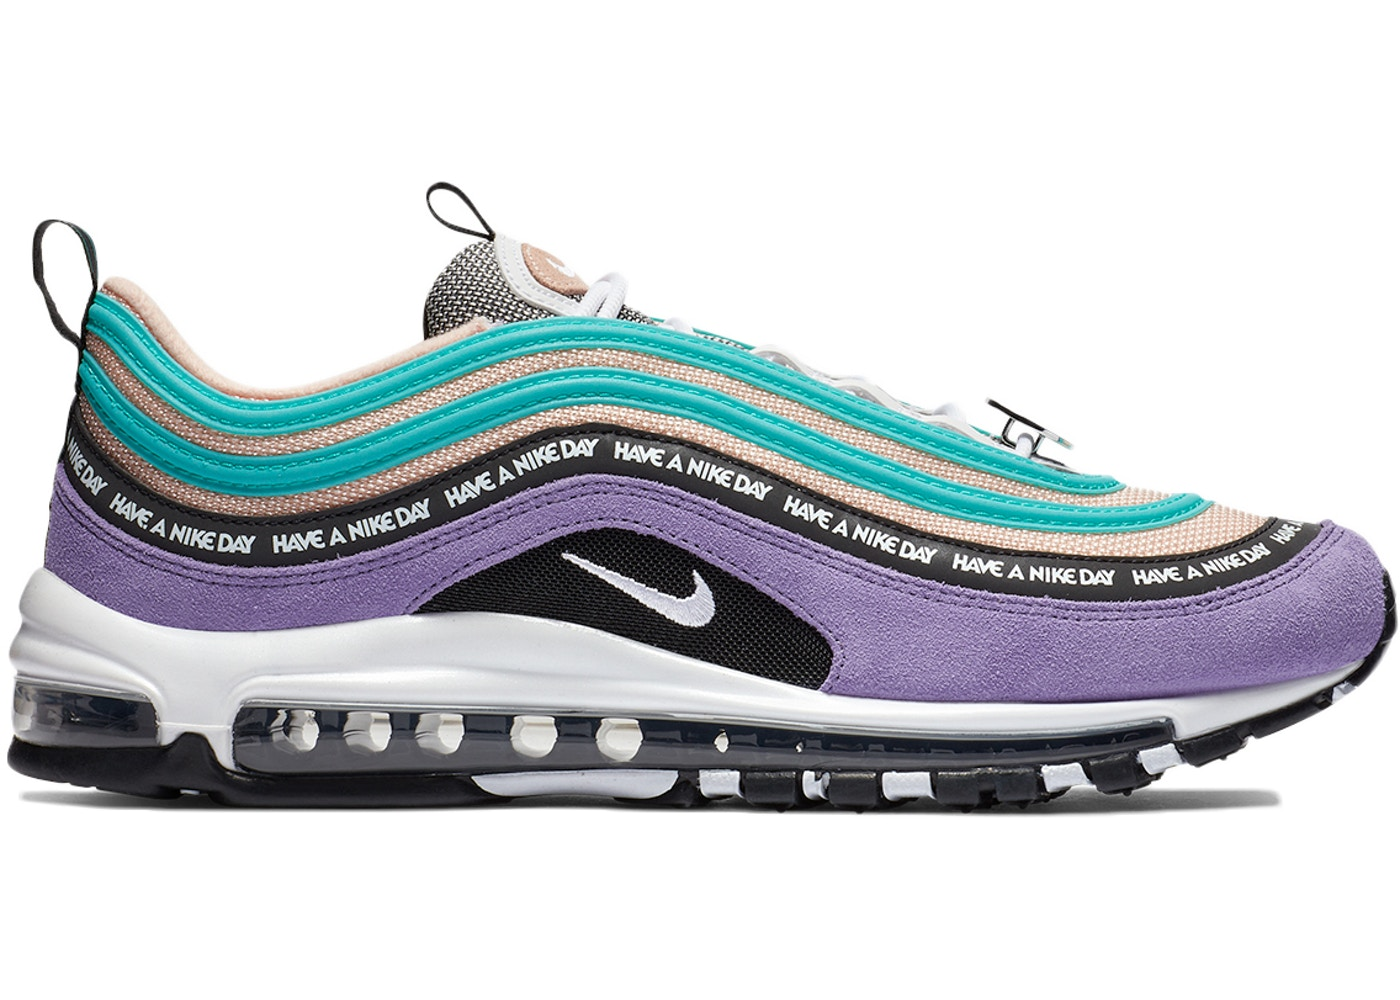
\includegraphics[width=1\textwidth]{airmax.jpg}
	\caption{My test image}
	\end{figure}
\end{document}